\scanpage{339}
\mspage{7}

final, et soit

\[
 p':\underset{\unsure{k|x|\downarrow}}{U'}\unsure{\mathbin{-}|\longrightarrow} U''
\]

l'inclusion, de sorte que

\[
 p'_!(e_{U'})=(p'p)_!(e_U)\unsure{=|\simeq} U'
 \quad\begin{gathered}\text{en tant qu'objet}\\
 \text{dans }U''^\wedge\ \text{(sans \deleted{\unsure{préf.}}\unsure{rapports|préf.}}\\
 \text{avec le préfaisceau}\\
 \text{final }e_{U''}\text{)}\end{gathered}
\]

Considérons

\diagram{\begin{tikzcd}[ampersand replacement=\&,column sep=large]
 U\arrow[r,hook,no head,"i"]\arrow[d,"p''=p'p"'] \& X\arrow[d,"q''"] \& T\arrow[l,hook',dashed,"j"']\arrow[d,"\mathrm{iso}"]\\
 U''\arrow[r,hook,"i''"']\arrow[ur,phantom,"\substack{\text{cocart.}\\\text{et cart.}}" description] \& X'' \& T''\arrow[l,hook',dashed,"j''"]
\end{tikzcd}}

Cette fois $U,X$ \uline{et} $U''$ sont $W_\infty$-asph. (et même contractiles toutes trois), \deleted{donc $i,p''$} \inserted{donc} $i,p''$ sont dans $W$, pourtant $X''$ n'est pas $W_\infty$-asph. (donc $i'',q''\notin W_\infty$), car pour qu'\unsure{el|il}\deleted{\unsure{le}} le soit \inserted{i.e. pour que $\unsure{i''|i'''}\in W_\infty$,} il faudrait (prop. 7, \unsure{cor|ou} page $85^*$) que \inserted{$i''$ soit \unsure{loc.|hom.} asph., i.e.} $U''_{/t''}$ soit $W_\infty$-asphérique. Mais par construction $U''_{/t''}\simeq U'$, qui n'est \uline{pas} $W_\infty$-asphérique.

% slanted
\margin{pas encore démontré !}

\figure{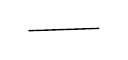
\begin{tikzpicture}\draw[line width=.5pt] (0,0) -- (.9,.03);\end{tikzpicture}}

Voilà un exemple encore plus simple d'un foncteur $f:\Psi\longrightarrow X$ tel que $f_!(e_\Psi)$ ne soit pas $W_\infty$-asphérique, \deleted{L'idée} i.e. d'un diagramme

\diagram{\begin{tikzcd}[ampersand replacement=\&,row sep=tiny]
 \& b\\
 a\arrow[ur,"\beta_0"]\arrow[dr,"\gamma_0"'] \&\\
 \& c
\end{tikzcd}}

% archive sheet number: 339
